% part I
% \titleformat{\chapter}
%   {\chap}{\thechapter}{1em}{}
% \titlespacing*{\chapter}{0pt}{3.5ex plus 1ex minus .2ex}{2.3ex plus .2ex}
%
\part{毕业论文(设计)}

\chapter{绪论(章的标题,三号仿宋加黑)}

\begin{equation}
\frac{a}{b}
\end{equation}

\section{节的标题(小三号仿宋加黑)}

\subsection{节的标题(四号仿宋加黑)}

\subsubsection{节的标题,仿宋四号加黑}
\cite{small}
\chapter{正文}

\begin{figure}[H]
    \centering
    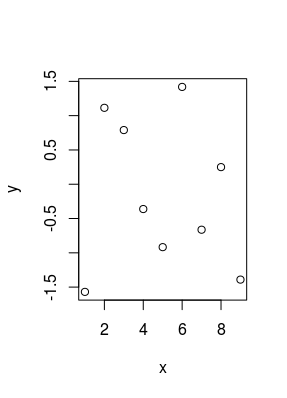
\includegraphics{../assets/sample.png}
    \caption{正态随机数}
\end{figure}

\section{节的标题(仿宋小三号加黑)}
\begin{equation}
\frac{1}{2}
\end{equation}
\subsection{节的标题(仿宋四号加黑)}

符号说明
{\wuhao
\begin{longtable}{p{5cm}p{5cm}}
\caption{符号说明}\\
\hline
项目内容 & 特点\\
\hline
模拟& 同方差\\
\hline
\end{longtable}
}
项目内容

\section{结论}

\printbibliography[heading=chapbib]